\documentclass[letterpaper, 10 pt, conference]{ieeeconf}
\IEEEoverridecommandlockouts
\overrideIEEEmargins{}
% Language
\usepackage[english]{babel}
% Graphics
\usepackage[pdftex]{graphicx}
\usepackage{adjustbox}
\graphicspath{{./figures/}}
\DeclareGraphicsExtensions{.pdf,.jpg,.jpeg,.png}
% Math
\usepackage[cmex10]{amsmath}
\usepackage{bm}
\interdisplaylinepenalty=2500{}
\usepackage{physics}
% Floats
\usepackage{booktabs,multirow}
\usepackage[caption=false,font=footnotesize]{subfig}
% Quotes
\def\enquote#1{``{#1}''}
% \def\enquote#1{\lq{#1}\rq}
% Tikz
\usepackage{tikz,pgfplots}
\pgfplotsset{compat=1.3}
% URLs
\usepackage{url}
% Ref commands
\newcommand{\fref}[1]{Fig.~\ref{#1}}
\newcommand{\sfref}[2]{\fref{#1}\,\subref{#2}}
\newcommand{\tref}[1]{Table~\ref{#1}}
\newcommand{\sref}[1]{Section~\ref{#1}}
% Math commands
\newcommand{\mdof}{\text{\ac{dof}}}

% Acronyms
\usepackage[acronym,shortcuts]{glossaries}
\glsdisablehyper
\newacronym{lrf}{LRF}{Laser Range Finder}
\newacronym{svd}{SVD}{Singular Value Decomposition}
\newacronym[longplural=Degrees of Freedom]{dof}{DoF}{Degree of Freedom}
\glsunset{dof}
% Definitions
\newtheorem{definition}{Definition}
\hyphenation{%
accel-era-tion
bi-manual
classi-cal
ma-nipu-la-tion
ma-nipu-la-tor
pa-rame-ters}

\title{\LARGE
  \textbf{SCALAR - Simultaneous Calibration of 2D Laser Range Finder Extrinsic Parameters And Robot Kinematics Using Three Planar Constraints}}

\author{Teguh Santoso Lembono, Francisco Su\'{a}rez-Ruiz, and Quang-Cuong Pham%
  \thanks{The authors are with the School of Mechanical and Aerospace
          Engineering, Nanyang Technological University, Singapore.}}

\begin{document}
\maketitle
\thispagestyle{empty}
\pagestyle{empty}

% Sections
\begin{abstract}
Industrial robots are increasingly used in various applications where the robot accuracy becomes very important, hence calibrations of the robot's kinematic parameters and the measurement system's extrinsic parameters are required. However, the existing calibration approaches are either too cumbersome or require another expensive external measurement system such as laser tracker or measurement spinarm. In this paper, we propose SCALAR, a calibration method to simultaneously improve the extrinsic parameters of a 2D \ac{lrf}, attached to the robot, and the robot's kinematic parameters. Three flat planes are placed around the robot, and for each plane the robot moves to several poses such that the \ac{lrf}'s ray intersect the respective plane. Geometric planar constraints are then used to optimize the calibration parameters using Levenberg-Marquardt nonlinear optimization algorithm. We demonstrate through simulations that SCALAR can reduce the position and orientation errors of the robot system from 21mm and 4$^o$ to 0.1mm and 0.02$^o$.  
\end{abstract}

%%% Local Variables:
%%% mode: latex
%%% TeX-master: "../main"
%%% End:

\section{Introduction}
\label{sec:introduction}

Robots have been used in many industrial applications, such as pick and place, spray-painting, and spot-welding. In those applications, the robots either do not need very high accuracy (such as in material handling for large objects), or the robots are programmed by teaching, where the important parameter is the repeatability of the robot instead of the accuracy. Repeatability refers to the capability of the robot to return to the same location as previously taught precisely, whereas accuracy refers to the capability of the robot to reach a location (computed based on the robot kinematics model) in the robot workspace. For tasks where the environment is very structured and the workpiece is always the same, the robot can be taught via a teaching pendant manually to reach the target locations once, and in such case the accuracy of the robot becomes irrelevant. 

However, there are a lot of interests to use robot on many other applications where the accuracy of the robot becomes very crucial, in which the robot has to adapt to each task automatically with a great precision. Consider, for example, a robot drilling task where the robot is supposed to drill several holes at precisely-defined locations on a workpiece, which can be different for each task. Programming by teaching in this case will require us to re-program the robot for each workpiece, which is very inefficient. If we want to program the robot automatically for such a task, the robot has to be able to do a few things accurately: the robot has to scan the workpiece, determine the location for the holes, and finally
move to that location precisely. The accuracy of such a robotic system depends on at least two things: The accuracy of the robot and the accuracy of the measurement system. 

The accuracy of the robot is determined by how closely the kinematic parameters of the robot model resemble the actual kinematic parameters of the physical robot. This is affected by the manufacturing process, the assembly process, and the wear and tear during the operation of the robot. A robot kinematics calibration is normally conducted to achieve a better accuracy, either by using an external measurement system (such as motion capture system or coordinate measuring machines) or by constraining the motion of the end effector.

The accuracy of the measurement system can be divided into two parts: the accuracy of the measurement device itself and the accuracy of the homogeneous transformation between the measurement frame to the robot frame. The accuracy of the measurement device depends on the type of device that is used and its specification. For example, a camera system is generallly less precise as compared to a laser system, although a camera can give more information. The second part of the accuracy comes from the fact that the data from a measurement system is always obtained in the measurement device coordinate frame, and it needs to be transformed to the robot coordinate system. Hence, the homogeneous transformation from the robot coordinate frame to the measurement device frame needs to be obtained. The homogeneous transformation matrix is often called the extrinsic parameters of the measurement device, and the method to estimate the extrinsic parameters is called the extrinsic calibration.  

In this paper we present SCALAR, a calibration method to simultaneously improve the accuracy of the robot and the measurement system. SCALAR uses a near-range 2D \ac{lrf}, attached to a robot, to calibrate the kinematics parameters of the robot and at the same time also calibrate the extrinsic parameters of the \ac{lrf}. \ac{lrf} is chosen because it gives very accurate measurement data both for the calibration and for the subsequent task (such as drilling).  

The overall calibration procedure is as follows:
\begin{enumerate}
\item The \ac{lrf} is attached to the robot, and three perpendicular planes are set around the robot. Only the rough estimate of the position and orientation of the planes are necessary to be known, so the setup can be easily done.
\item For each plane, the robot is moved to several poses such that the \ac{lrf}'s 2D ray is projected onto the plane. The data from the \ac{lrf} as well as the joint angles information are collected.
\item An optimization algorithm (Levenberg-Marqueadt) is used to find the optimal robot kinematics parameters together with the \ac{lrf} extrinsic parameters by satifsfing the following constraints: the projected \ac{lrf} data should fall on the three planes. 
\end{enumerate}

The remainder of the paper is as follows. In \sref{sec:related}, we discuss the existing approaches to the calibration problem, both for the robot kinematics and the \ac{lrf} extrinsic parameters, and how SCALAR differs from the others. In \sref{sec:method}, SCALAR is explained in detail. A simulation study is presented in \sref{sec:simulation} to verify the method, and finally we conclude with a few remarks in \sref{sec:conclusions}.  



\renewcommand{\arraystretch}{1.5}
\begin{table*}[htp]
\caption{Examples of Unconstrained Calibration}
\label{tab:unconstrained_calib}
\centering
\begin{tabular}{c c c c c}
\toprule
\textbf{Researchers} &  \textbf{Robot} & \textbf{Measurement Device} &  \textbf{Initial Accuracy[mm]}  & \textbf{Final Accuracy[mm]}\\
\midrule
Ginani and Mota \cite{Ginani2011} & ABB IRB 2000 & ROMER Measurement Arm & 2.20 & 1.40 \\
Ye et al. \cite{Ye2006} & ABB IRB 2400/L & Faro Laser Tracker & 1.764 & 0.640 \\
Nubiola and Bonev \cite{Nubiola2013} & ABB IRB 1600-6/1.45 & Faro Laser Tracker ION & 2.158 & 0.696 \\ 
Newman et al. \cite{Newman2000} & Motoman P-8 & SMX Laser Tracker & 3.595 & 2.524\\
\bottomrule
\end{tabular}
\end{table*}

\section{Related works}
\label{sec:related}
\subsection{Calibration of robot kinematic parameters}
\label{sec:kine_calib}



Robot kinematics calibration has been researched for a long time; some of the earliest works began in 1980s. The calibration procedures can be categorized into unconstrained and constrained calibration. In unconstrained calibration, the robot moves its end-effector to several poses while an external measurement system measures the pose. The measured pose is then compared to the one computed from the kinematics model, and the model is updated to minimize the difference between the predicted pose and the measured pose. In constrained calibration, some constraints are applied to the motion of the end effector, and the constraints yield several calibration equations by which the robot kinematics parameters are calibrated. 


Examples of unconstrained calibration works can be seen in \tref{tab:unconstrained_calib}. The issues with such calibration method are the difficulty in setting up the calibration setup and the expensive cost of the external measurement system. For example, the cost of a laser tracker is more than $\$100,000$ \cite{Nubiola2013}. Therefore, many researchers try to find calibration methods which only rely on the internal sensors of the robot by constraining the motion of the end effectors, such as in constrained calibration. 

In \cite{Ikits1997}, Ikits and Hollerbach propose a kinematic calibration method using a planar constraint. The robot end effector (a touch probe) is moved to touch random points on a plane. When the touch probe is in contact with the plane, the joint angles are recorded. The kinematics parameters of the robot model are then updated to satisfy the planar constraint. While the approach is promising, they also report that some of the parameters are hardly observable when the measurements are noisy or when the model is not complete. The unobservability of the parameters means that some of them cannot be obtained accurately from the calibration procedure.

In \cite{Zhuang1999}, Zhuang et al. investigate robot calibration with planar constraints, in particular the observability conditions of the robot kinematic model parameters. They prove that a single-plane constraint is insufficient for calibrating a robot, and a minimum of three planar constraints are necessary. Using three planar constraints, the constrained system is proved to be equivalent to an unconstrained point-measurement system under three conditions: a) All three planes are mutually non-parallel, b) the identification Jacobian of the unconstrained system is nonsingular, and c) the measured points from each individual plane do not lie on a line on that plane. They verify the theory by doing a simulation on a PUMA560 robot. 

In \cite{Joubair2015}, Joubair and Bonev calibrated both the kinematic and non-kinematic (stiffness) parameters of a FANUC LR Mate 200iC industrial robot by using planar constraints, in the form of a high precision 9-inches granite cube. The robot is equipped with an MP250 Renishaw touch probe, which is then moved to touch four planes of the granite cube. The granite cube's face is flat to within 0.002mm. They improved the maximum plane error from 3.740mm to 0.083mm. 

\subsection{Calibration of extrinsic 2D \ac{lrf} parameters}
\label{sec:laser_calib}
Extrinsic calibration of an \ac{lrf} consists of finding the correct homogeneous transformation from the robot coordinate frame to the laser coordinate frame. Most of the works on extrinsic calibration of an \ac{lrf} involves a camera, since both sensors are often used together in many applications. The works in this field are largely based on Zhang and Pless' work \cite{Zhang2004}. They propose a method to calibrate both a camera and an \ac{lrf} using a planar checkerboard pattern. First, the camera is calibrated by using a checkerboard pattern, using a standard hand-eye calibration procedure. The calibrated camera is then used to calculate the pose of the pattern. Next, the robot is moved to several poses with the \ac{lrf} pointing to the pattern. By using the geometric constraints that all the data points from the \ac{lrf} should fall on the pattern plane, the extrinsic parameters of the \ac{lrf} can be obtained. Finally, the same constraints is used to optimize both the intrinsic and extrinsic parameter of the camera and the extrinsic parameter of the \ac{lrf}. The nonlinear optimization problem is solved by using the Levenberg-Marquardt optimization algorithm.

Unnikrishnan and Hebert \cite{Unnikrishnan2005} use the same setup as \cite{Zhang2004}, although they do not optimize the camera parameter simultaneously due to the nonlinearity of the resulting cost function. 
Li et al. \cite{Li2007} use a specially designed checkerboard to calibrate the extrinsic parameters between a camera and an \ac{lrf}, and claim that the result is better than \cite{Zhang2004}. Vasconcelos et al. \cite{Vasconcelos2012} develop a minimal closed-form solution for the extrinsic calibration of a camera and an \ac{lrf}, based on the work in \cite{Zhang2004}. 


SCALAR can be seen as a combination of the algorithm for extrinsic calibration of an \ac{lrf} \cite{Zhang2004} and the algorithm for calibration of robot kinematics parameter using three planar constraints \cite{Joubair2015}. It has the following advantages as compared to the other calibration approaches:
\begin{enumerate}
\item SCALAR simultaneously calibrates both the \ac{lrf} extrinsic parameters and the robot kinematics parameters. As calibration process is often cumbersome, this saves a lot of time and effort.
\item SCALAR does not need an additional camera to calibrate the \ac{lrf}, unlike \cite{Zhang2004}.
\item SCALAR does not need another expensive external measurement system. The measurement is done using the \ac{lrf} that will also be used in the robot task, hence it does not incur additional cost. Moveover, an \ac{lrf} can achieve very high accuracy at much lower cost as compared to the commonly used measurement systems such as Vicon or Faro Laser Tracker. 
\item SCALAR does not need a precisely manufactured calibration object such as the granite cube in \cite{Joubair2015}, which requires the planes' position and orientation to be known accurately. SCALAR only requires
three flat surfaces which are oriented roughly perpendicular to each other and the rough estimate of their locations. This also means that the calibration setup can be done easily.
\item The calibration poses can be distributed throughout the whole workspace, instead of being confined only in a local region such as in \cite{Joubair2015}. 
\end{enumerate}



%%% Local Variables:
%%% mode: latex
%%% TeX-master: "../main"
%%% End:

\section{Method}
\label{sec:method}
\begin{figure}[t]
  \centering
  \vspace*{2mm}
  \subfloat[]{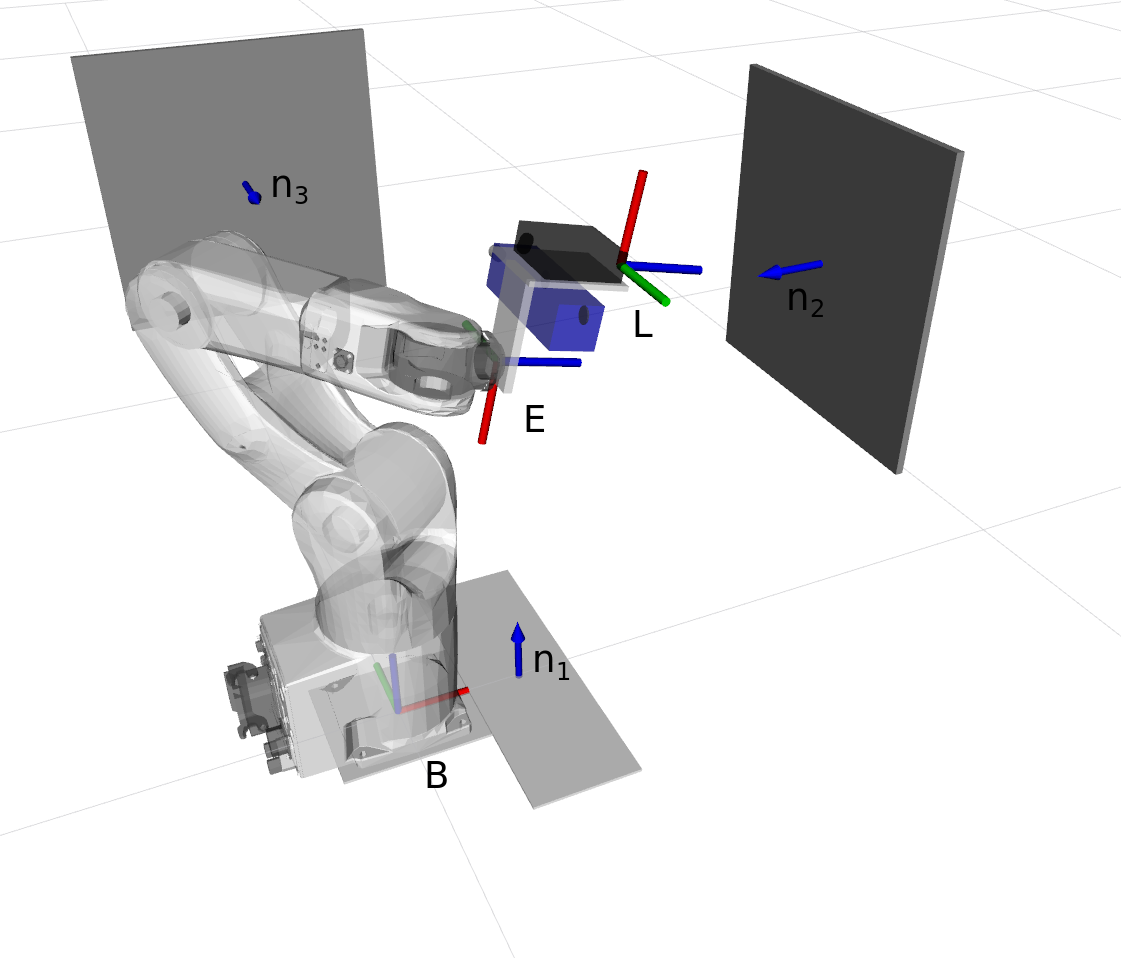
\includegraphics[height=60mm]{robot_setup}}
  \caption{Robot setup for the calibration}
  \label{fig:robot_setup}
\end{figure}


\renewcommand{\arraystretch}{1.5}
\begin{table}[htp]
\caption{Robot DH Parameters}
\label{tab:dh_params}
\centering
\begin{tabular}{c c c c c}
\toprule
i &  \textbf{$\alpha_i$} & \textbf{$a_i$} &  \textbf{$\theta_i$}  & \textbf{$d_i$}\\
\midrule
1 & 0.0 & 0.0 & 0.0 & 345.0\\
2 & -90.0 & 0.0 & -90.0 & 0.0\\
3 & 0.0 & 305.0 & 90.0 & 0.0\\
4 & 90.0 & -10.0 & 0.0 & 300.0\\
5 & -90.0 & 0.0 & 0.0 & 0.0\\
6 & 90.0 & 0.0 & 0.0 & 70.0\\
\bottomrule
\end{tabular}
\end{table}

The calibration setup is depicted in \fref{fig:robot_setup}, where three perpendicular planes ($k=1,2,3$) are installed around the robot. An \ac{lrf} is attached on the robot flange. For each plane, the robot is moved to $N$ poses such that the \ac{lrf} is directed to the respective plane. One data set from the \ac{lrf} consists of hundreds of data points, so $M$ data points are selected randomly from the \ac{lrf} data for each pose, together with the joint angles of the robot. 

This section provides the detail on how to calibrate both the extrinsic parameters of the LRF and the robot kinematics parameters. First, the initial estimate of the LRF extrinsic parameter is obtained by using the linear least-square method based on the data from one of the planes. After that, the LRF extrinsic parameters and the robot kinematics parameters are optimized simultaneously to satisfy the three planar constraints, by using the Levenberg Marquardt nonlinear optimization method. At the end of this section, we explain how we can use \ac{svd} to analyse which calibration parameters are identifiable, and the steps to handle the unidentifiable parameters are then presented. 
\subsection{Obtaining the Initial Estimate of the \ac{lrf} Extrinsic Parameters}
\label{sec:first_step}
To obtain an initial estimate of the \ac{lrf} extrinsic parameters, only the data from one plane is necessary. Arbitrarily, the bottom plane $plane 1$ is chosen. The extrinsic parameters of the \ac{lrf} ${^E}\vb*{T}_L$, i.e. the homogeneous transformation from the robot flange coordinate frame to the \ac{lrf} coordinate frame, is estimated by the following calculation. 

Let the subscript/superscript $B$, $E$, and $L$ denote the coordinate frame of the robot base, the robot flange, and the \ac{lrf}, while the subscript $i$ and $j$ refer to the \ac{lrf} data point index and the robot pose index respectively. Let $\vb*{p}_{ji}$ be one of the data points from the \ac{lrf} which lies on the $plane 1$, $\vb*{n}_1$ be the normal unit vector of $plane 1$, and $d_1$ be the perpendicular distance from the origin of the robot coordinate system to $plane 1$.  Since $\vb*{p}_1$ is located on the $plane 1$, it has to satisfy the following constraint:
  \begin{equation}
  \label{eq:1}
  ({^B}\vb*{n}_1) ^T ({^B}\vb*{p}_{ji}) - {^B}d_1 = 0
   \end{equation}
${^B}\vb*{p}_{ji}$ depends on the robot pose ${^B}\vb*{T}_{E,j}$ at pose index j and the \ac{lrf} extrinsic parameter ${^E}\vb*{T}_L$, so \eqref{eq:1}  can be expanded,
  \begin{equation}
  ({^B}\vb*{n}_1) ^T ({^B}\vb*{T}_{E,j}) ({^E}\vb*{T}_L) ({^L}\vb*{p}_{ji}) - {^B}d_1 = 0
  \end{equation}.
${^B}\vb*{n}_1$ and $^{B}d_1$ are known approximately ($[0 \; 0\; 1\;0]$ and $0.0$), ${^B}\vb*{T}_{E,j}$ can be computed from the robot's joint angles at pose index $j$, and ${^L}\vb*{p}_{ji}$ is obtained from the laser. Let $\vb*{n}^{'}_j = ({^B}\vb*{n}_1) ^T ({^B}\vb*{T}_{E,j}) = 
\left[n^{'}_{j,1} \quad n^{'}_{j,2} \quad n^{'}_{j,3}  \quad n^{'}_{j,4} \right]$, then  
  \begin{equation}
  \label{eq:3}
  (\vb*{n}^{'}_j) ^T ({^E}\vb*{T}_L) ({^L}\vb*{p}_{ji}) - {^B}d_1 = 0
  \end{equation}
The only unknown in \eqref{eq:3} is ${^E}\vb*{T}_L$ which has 12 elements $r_{uv}$, where u and v denote the column and the row index of the matrix. Note that the fourth row of ${^E}\vb*{T}_L$ only consists of 0 and 1. 
Without any loss of generality, let's assume that the data points from the \ac{lrf} lies on the XZ planes in the laser frame $L$, so ${^L}\vb*{p}_{ji} = \left[{^L}p_{i,x} \quad 0 \quad {^L}p_{i,z}\quad 1\right]$. If we expand \eqref{eq:3} and rearrange such that the components of ${^E}\vb*{T}_L$ are stacked together as a vector $\vb*{\Phi}_L$, we have
\begin{equation}
\label{eq:4}
  (\vb*{x}_{ji})  ^T (\vb*{\Phi}_L) = {^B}d_1 -  n^{'}_{j,4}
\end{equation}
, where 
\begin{multline}
  \vb*{x}_{ji} = \left[{^L}p_{i,x}\;n^{'}_{j,1} \quad {^L}p_{i,x}\;n^{'}_{j,2}\quad {^L}p_{i,x}\;n^{'}_{j,3}\quad  {^L}p_{i,z}\;n^{'}_{j,1}\right. \\ 
\left. {^L}p_{i,z}\;n^{'}_{j,2}\quad {^L}p_{i,z}\;n^{'}_{j,3} \quad n^{'}_{j,1} \quad n^{'}_{j,2} \quad n^{'}_{j,3} \right]
\end{multline}, 
and
\begin{multline}
  \vb*{\Phi}_L= \left[r_{11} \quad r_{21} \quad r_{31} \quad r_{13} \quad r_{23} \quad r_{33} \quad r_{14} \quad r_{24}  \quad r_{34} \right] 
\end{multline}
For each data point i, we obtain such equation as in \eqref{eq:4}. With $M$ data points per pose and a total of $N$ robot poses, we have $MN$ such equations. The equations can be stacked together to form the following matrix equation:
\begin{equation}
\label{eq:7}
  \vb*{X}   \vb*{\Phi}_L= \vb*{D}
\end{equation}
where 
\begin{equation}
\vb*{X} =\begin{bmatrix}
{\vb*{x}_{11}}^T \\ {\vb*{x}_{12}}^T  \\ \cdots\\{\vb*{x}_{1M}}^T \\ {\vb*{x}_{21}}^T \\ \cdots\\ {\vb*{x}_{2M}}^T  \\ \cdots \\ {\vb*{x}_{NM}}^T 
\end{bmatrix} \;, \; \vb*{D} =\begin{bmatrix}
{^B}d_1 -  n^{'}_{1,4} \\ {^B}d_1 -  n^{'}_{1,4}  \\ \cdots\\ {^B}d_1 -  n^{'}_{1,4}  \\ {^B}d_1 -  n^{'}_{2,4} \\ \cdots\\ {^B}d_1 -  n^{'}_{2,4}  \\ \cdots \\{^B}d_1 -  n^{'}_{N,4} 
\end{bmatrix}
\end{equation}
Equation \eqref{eq:7} can be solved by linear least square procedure to obtain $\vb*{\Phi}_L$. ${^E}\vb*{T}_L$ can then be computed as follows:
\begin{enumerate}
\item The parameters $[r_{11}, r_{21}, r_{31}]$ and $[r_{13}, r_{23}, r_{33}]$ are supposed to be unit vectors, so they should be normalized. They consistute the first and the third column of the matrix ${^E}T_L$
\item The parameters $[r_{14}, r_{24}, r_{34}]$ constitutes the position component of the matrix ${^E}T_L$, or its fourth column
\item The parameters $[r_{12}, r_{22}, r_{32}]$ can be calculated as the cross product of  $[r_{13}, r_{23}, r_{33}]$ and $[r_{11}, r_{21}, r_{31}]$ 
\end{enumerate}

To use the extrinsic parameters ${^E}\vb*{T}_L$ for the subsequent step, 9 parameters would be too redundant. Therefore, we choose the axis-angle representation for the rotation part of ${^E}T_L$ which gives us 4 parameters $[r_x, r_y, r_z, r_{\theta}]$, and 3 more parameters for the location part $[p_x, p_y, p_z]$. 


\subsection{Optimizing both the \ac{lrf} Extrinsic Parameters and Robot Kinematic Parameters}
\label{sec:second_step}
In the second step, the data from all the three planes are used to optimize the parameters of the \ac{lrf}, robot kinematics, as well as the plane parameters. The objective function is described as follows:

\begin{equation}
 f (\vb*{\Phi}) =  \sum_{k=1}^{3} \sum_{j=1}^{N} \sum_{i=1}^{M} (({^B}\vb*{n}_1) ^T ({^B}\vb*{p}_{ji}) - {^B}d_1)^2
\end{equation}

The parameters $\vb*{\Phi}$ consists of the followings:
\begin{enumerate}
\item Robot kinematics parameters. We choose the modified DH parameters \cite{Hayati1985} $[a_i \;, \alpha_i \;,\theta_i \;,d_i], i=1, 2, \cdots ,6$ to represent the robot kinematics, so we have 6*4 = 24 DH parameters for a 6 \ac{dof} robot arm (refer to \tref{tab:dh_params}). 
\item Laser extrinsic parameters. As mentioned in the previous section, we use the axis angle representation for the rotation part $[r_x, r_y, r_z, r_{\theta}]$,and the location is represented by 3 numbers $[p_x, p_y, p_z]$. 
\item Plane parameters. Each plane has 4 parameters $[n_{k,x}, n_{k,y}, n_{k,z}, d_{k}]$, 3 for the unit vector and 1 for the distance, so we have 4*3 = 12 parameters. 
\end{enumerate}

In total, we have 43 parameters to be optimized by minimizing the objective function $f{\Phi}$. To do that, we need to ensure that the number of data points $MN$ exceeds the number of parameters. The optimization problem is then solved by using Levenberg-Marquardt nonlinear optimizer \cite{Newville2014}. For the unit vector parameters ($[r_1, r_2, r_3]$ and  $[n_{k,x}, n_{k,y}, n_{k,z}]$), the following constraints are added to the solver:
\begin{equation}
\label{eq:10}
{r_z} = \sqrt{1 - {r_x}^2 - {r_y}^2}
\end{equation}
\begin{equation}
\label{eq:11}
n_{k,z} = \sqrt{1 - {n_{k,x}}^2 - {n_{k,y}}^2}
\end{equation}


The objective function $f(\vb*{\Phi})$ basically uses the constraints that all data points from the \ac{lrf} have to be on the respective plane. \cite{Zhuang1999} proved that such constraints are essentially equivalent to the calibration of a robot using end-point measurement. Further analysis on the observability of the parameters will be presented on the next section. 

\subsection{The identifiability of the calibration parameters}
\label{sec:third_step}

Depending on the chosen robot calibration poses and the choices of the parameters, some of the calibration parameters might not be observable, due to the redundancy among the parameters. This is a critical problem in calibration, as it will result in some of the parameters assuming erratic values and unstable calibration result. To prevent that, we have to first analyse which calibration parameters are identifiable and which are not. 

Following the approach in \cite{Hollerbach1996} and \cite{Joubair2015}, SVD is applied on the identification Jacobian matrix $\vb*{J}$. $\vb*{J}$ can be computed as follows. Let  $f_{kji}(\Phi)$ be the constraint equation on one of the data point $i$ at the robot pose $j$ and on the plane k:
\begin{equation}
 f_{kji}(\Phi) =  ({^B}\vb*{n}_k) ^T ({^B}\vb*{p}_{ji}) - {^B}d_k
\end{equation}
Then $vb*{J}$ can be computed by differentiating all the data points $i = 1, \cdots, M$ for all the poses $j = 1, \cdots, N$ and for all the planes $k=1,2,3$, and stack them together as a matrix:

\renewcommand\arraystretch{1.5}
\begin{equation}
\vb*{J} = \begin{bmatrix}
 \frac{\partial f_{111}(\Phi)}{\partial\Phi}\\
 \frac{\partial f_{112}(\Phi)}{\partial\Phi}\\
 \cdots \\
 \frac{\partial f_{3MN}(\Phi)}{\partial\Phi}\\
	\end{bmatrix}
\end{equation}

We can then apply SVD on matrix $\vb*{J}$:

\begin{equation}
 \vb*{J} = \vb*{U}\vb*{\Sigma}\vb*{V}^T
\end{equation}
Note that for this identification step, the parameters $[r_z, n_{1,z}, n_{2,z}, n_{3,z}]$ are excluded from the parameter vector $\Phi$, since those four parameters are obtained as linear combinations of other parameters (Equation \eqref{eq:10} and \eqref{eq:11}). That leaves us with 43-4 = 39 parameters in $\vb*{\Phi}$, which correlates to the 39 singular numbers in $\Sigma$. The number of singular values with the value of zero in $\Sigma$ is then equal to the number of unidentifiable parameters. For a given zero-value singular number $\sigma_r$, the rth column vector of matrix $\vb*{V}$ is the linear combination of the parameters $\vb*{\Phi}$ which cannot be identified independently. 
In our case, out of the 39 parameters, there are 7 redundant parameters. By analysing the matrix $\vb*{V}$, those 7 redundant parameters are due to:
\begin{enumerate}
\item The parameters $d_6$ (the translation along the z-axis of the 6th link frame on the flange) and $p_z$ (the z coordinate of the \ac{lrf} frame) are redundant. This has obvious physical meaning, because if we shift the origin of the frame 6 in its z direction, we can compensate by shifting the origin of the \ac{lrf} frame in the opposite direction
\item The parameters $\theta_6$ and $r_\theta$ are redundant. These are the rotation of the last link and the rotation of the \ac{lrf} frame, both around the same z-axis. 
\item The parameters $d_2$ and $d_3$ are redundant. We can shift the frame 2 in its z direction, and compensate by shifting the frame 3 in the other direction. 
\item Lastly, we have four redundant parameters as the linear combination of the DH parameter of the first link ($a_1, \alpha_1, \theta_1, d_1$) and all the three planes' parameters. Physically, this relates to the fact that we can adjust the location of the base frame freely by changing the value of ($a_1, \alpha_1, \theta_1, d_1$), and all the planes' parameters will adjust according to the new base location. In other words, the base coordinate is not constrained, or it is "floating"
\end{enumerate}

For each pair of the redundant parameters, we can assign a fix value to one of the parameters. In this case, we set the value of the parameters [$d_6, \theta_6, d_2, a_1, \alpha_1, \theta_1, d_1$] to maintain their initial model's values. 

\section{Simulation}
\label{sec:simulation}

We verify SCALAR through simulation of the calibration procedure. The simulation is conducted by using Robot Operating System and Gazebo where the robot model, the \ac{lrf}, and the three planes can be simulated.  
As shown in \fref{fig:robot_setup}, three perpendicular planes are located around the robot, and the robot is moved such that the \ac{lrf} ray intersects each plane. Simulated data from the \ac{lrf} can be obtained and Gaussian noise can be added to the data. The data is then used as input to the calibration procedure. 

After the calibration procedure, the robot is moved to 10000 random poses to evaluate the proposed calibration method. Let ${^B}\vb*{T}_{L,j,true}$ and ${^B}\vb*{T}_{L,j,model}$ be the true and calibrated pose of the \ac{lrf} frame w.r.t. the robot base frame at the robot pose index $j$, respectively, then the error of the calibrated model can be computed as follows. 
\begin{equation}
\Delta \vb*{T}_j =  {{^B}\vb*{T}_{L,j,model}}^{-1} \cdot\; {^B}\vb*{T}_{L,j,true}
\end{equation}
Let $\delta t_{uv}$ be the element of $\Delta \vb*{T}_j$ with the subscript $u$ and $v$ refer to the row and column index, then the position error at the robot pose index $j$, $\delta p_j$, can be computed by
\begin{equation}
\delta p_j = \sqrt{\delta t_{14}^2 + \delta t_{24}^2 + \delta t_{34}^2} \quad .
\end{equation}
Let $\delta \vb*{R}_j$ be the rotation part of the homogeneous transformation matrix $\Delta \vb*{T}_j$. $\delta \vb*{R}_j$ can be represented by using an axis-angle notation, $[r_{j,1}\quad r_{j,2}\quad r_{j,3}\quad \delta \theta_j]$. We use $\delta\theta_j$ as the orientation error at the robot pose index $j$.  $\delta\theta_j$ can be seen as the amount of rotation necessary to rotate the calibrated pose to the true pose. The errors $\delta p_j$ and $\delta\theta_j$ are then averaged over the 10000 random poses.

The simulated robot's kinematic model is considered as having the true kinematic parameters, and the initial kinematic model is generated by introducing random Gaussian errors to the true parameters within the range of $\pm$ 2mm and $\pm$ 1$^o$ for the linear and angular parameters, respectively. Note that the errors are intentionally set to be large to illustrate the robustness of the calibration method. By using the proposed error formulation, the average errors of this initial kinematic model as compared to the true model are 21mm and 4$^o$.


\begin{figure}[t]
  \centering
  \subfloat{\includegraphics[height=40mm]{laser_pos}}
  \subfloat{\includegraphics[height=40mm]{laser_ori}}
  \caption{The effect of the measurement noise towards the position and orientation error} 
  \label{fig:laser_noise}
\end{figure}


\begin{figure}[t]
  \centering
  \subfloat{\includegraphics[height=40mm]{num_of_poses_pos}}
  \subfloat{\includegraphics[height=40mm]{num_of_poses_ori}}
  \caption{The effect of the number of poses towards the position and orientation error} 
  \label{fig:num_of_poses}
\end{figure}


\begin{figure}[t]
  \centering
  \subfloat{\includegraphics[height=40mm]{num_of_points_pos}}
  \subfloat{\includegraphics[height=40mm]{num_of_points_ori}}
  \caption{The effect of the number of points towards the position and orientation error} 
  \label{fig:num_of_points}
\end{figure}

\begin{figure}[t]
  \centering
  \subfloat{\includegraphics[height=40mm]{plane_param_linear_pos}}
  \subfloat{\includegraphics[height=40mm]{plane_param_linear_ori}}
  \caption{The effect of the plane parameters initial position estimate error towards the position and orientation error} 
  \label{fig:plane_params_linear}
\end{figure}

\begin{figure}[t]
  \centering
  \subfloat{\includegraphics[height=40mm]{plane_param_angular_pos}}
  \subfloat{\includegraphics[height=40mm]{plane_param_angular_ori}}
  \caption{The effect of the plane parameters initial orientation estimate error towards the position and orientation error} 
  \label{fig:plane_params_angular}
\end{figure}




\subsection{The effect of the measurement noise}
\label{sec:meas_accuracy}
The accuracy of the calibration procedure greatly depends on the accuracy of the measurement system, which is affected by the noise on the data. In this section, Gaussian noises with zero means and varying standard deviations $\sigma_{\rm{noise}}$ are added to the measurement data in the simulation, and its effect on the calibration errors is shown in \fref{fig:laser_noise}. As $\sigma_{\rm{noise}}$ decreases, the calibration errors decrease. At $\sigma_{\rm{noise}}$ = 0.1mm, the position and orientation errors are around 0.1mm and 0.02$^o$, respectively. For the subsequent sections, $\sigma_{\rm{noise}}$ is set at 0.1mm. 

\subsection{The effect of the number of calibration poses}
\label{sec:calib_poses}
For each plane, the robot is moved to $N$ poses, so in total we have $3N$ calibration poses. At each pose, we select $M$ data points from the \ac{lrf} data. In this section we evaluate the effect of $3N$ and $M$ to the calibration errors. In \fref{fig:num_of_poses}, it can be seen that as the number of poses $3N$ increases, the error decreases until around $3N$=60, beyond which it does not change much. It can be concluded that 60 robot poses are sufficient to calibrate the robot model accurately. 


Similarly, we can see from \fref{fig:num_of_points} that as $M$ increases the calibration errors decrease. After around 10 points, the calibration errors do not change significantly. Therefore, although an \ac{lrf} can give more than 300 data points per robot pose, using more than 10-20 points does not improve the calibration by much. 



\subsection{The effect of the plane parameters' initial estimate}
\label{sec:plane_params}
One of the advantages of SCALAR is that the planes parameters do not need to be precisely known. Here we vary the planes parameters estimate to demonstrate the robustness of our method. The initial estimates of the normals and the positions of the planes are disturbed by as much as 30$^o$ and 65mm, as shown in \fref{fig:plane_params_linear} and \fref{fig:plane_params_angular}. From the figure, it can be seen that the position and orientation error are not affected by the errors in the planes parameters initial estimate. In fact, after calibration, the planes' parameters in the calibrated model approach the true parameters within 0.1mm and 0.02$^o$.






\section{Conclusions}
\label{sec:conclusions}

In this paper, we have proposed a method to calibrate simultaneously a 2D \ac{lrf} extrinsic parameters and a 6\ac{dof} robot kinematics by using just three flat planes, arranged perpendicularly towards each other around the robot. The proposed method is much easier to implement than the previous methods in the literature, as it does not require other expensive measurement system or tedious setup. Through the simulation, we have also verified that the method can reduce the error in position and orientation from (21mm, 4$^o$) to (0.1mm, 0.02$^o$), respectively. This is very useful for many industrial robotics applications that require great accuracy. The method will be implemented on the real robot, and we will present the result in the next work. 



\section*{Acknowledgment}
This work was supported in part by NTUitive Gap Fund NGF-2016-01-028
and SMART Innovation Grant NG000074-ENG.


% You can use one of these two commands to balance the last page columns
\IEEEtriggeratref{7}
% \IEEEtriggercmd{\enlargethispage{-100mm}}
\bibliographystyle{IEEEtran}
\bibliography{IEEEabrv,references}

\end{document}

%%% Local Variables:
%%% mode: latex
%%% TeX-master: t
%%% End:
